\documentclass{article}
\usepackage[utf8]{inputenc}
\usepackage{multicol}
\setlength\columnsep{20pt}
\usepackage{listings}
\usepackage{geometry}
\usepackage{color}
\usepackage{float}
\setlength{\belowcaptionskip}{-10pt}
\setlength{\abovecaptionskip}{-30pt}
\floatstyle{boxed} 
\restylefloat{figure}
\usepackage{hyperref}
\usepackage{graphicx}
\definecolor{codegreen}{rgb}{0,0.6,0}
\definecolor{codegray}{rgb}{0.5,0.5,0.5}
\definecolor{codepurple}{rgb}{0.58,0,0.82}
\definecolor{backcolour}{rgb}{0.95,0.95,0.92}

\lstdefinestyle{mystyle}{
	backgroundcolor=\color{backcolour},   
	commentstyle=\color{codegreen},
	keywordstyle=\color{blue},
	numberstyle=\tiny\color{codegray},
	stringstyle=\color{codepurple},
	basicstyle=\footnotesize,
	breakatwhitespace=false,         
	breaklines=true,                 
	captionpos=b,                    
	keepspaces=true,                 
	numbers=left,                    
	numbersep=5pt,                  
	showspaces=false,                
	showstringspaces=false,
	showtabs=false,                  
	tabsize=2
}

\lstset{style=mystyle}
\title{Machine Learning\\ Home Work 03}
\author{aqeel labash}
\date{21 February 2016}
\geometry{
	a4paper,
	total={170mm,257mm},
	left=10mm,
	top=5mm,
}
\begin{document}

	\maketitle
		\textbf{This is The Third Home work which were decided (after second practice session) the home work link is \href{https://courses.cs.ut.ee/MTAT.03.227/2016_spring/uploads/Main/home-exercises-3.pdf}{ here} }
\begin{multicols*}{2}
{\centering \section*{First Question}}
{\centering\subsection*{A}}
To build the matrix I build the following code:
\begin{lstlisting}[language=R]
#Create y=X*B
#create (1,x) data columns
X<-cbind(rep(1,nrow(data)),data$x)
ypredict.mat<-X %*% beta
#Draw The points with two types of prediction
ypred.lm <- predict(linear.model, newdata = data)
plot(data)
points(data$x, ypredict.mat, col = "red")
points(data$x, ypred.lm, pch = 18, col = "blue")
\end{lstlisting}
To test the accuracy I draw the points on the graph by using the following code:
\begin{lstlisting}[language=R]
#Draw The points with two types of prediction
plot(data)
points(data$x, ypred, col = "red", lwd = 2)
ypred.lm <- predict(linear.model, newdata = data)
points(data$x, ypred.lm, pch = 18, col = "blue")
\end{lstlisting}
Figure 1 was the result and we can notice that points overlap :
\begin{figure}[H]
\begin{center}
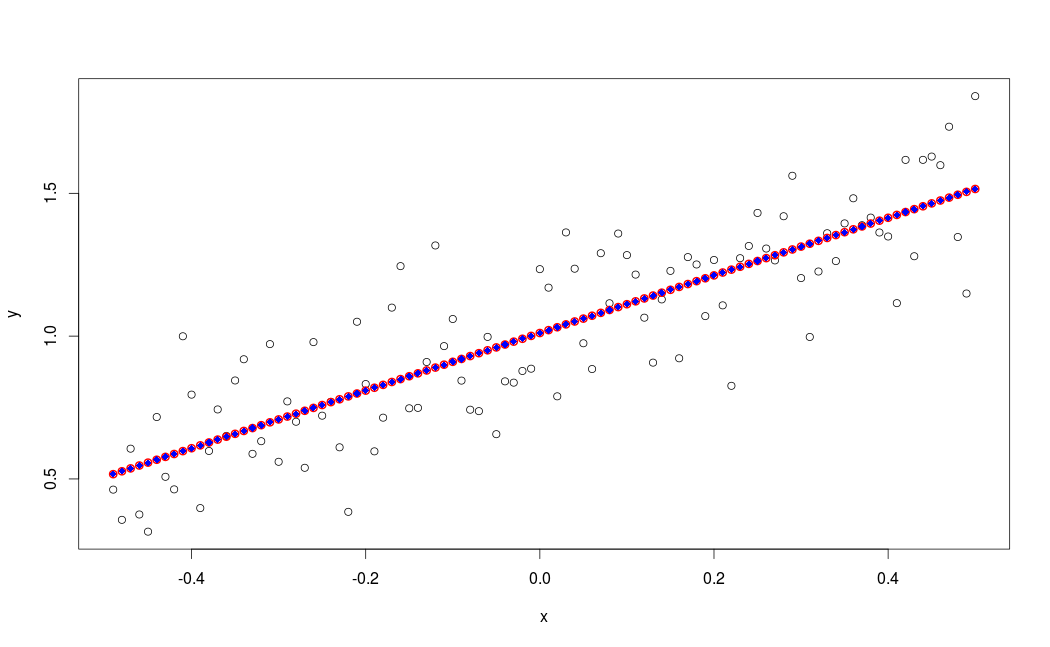
\includegraphics[scale=0.23]{plotpredictioncomparision.png}
\end{center}
\caption{Matrix vs predict function prediction}
\end{figure}
For more accuracy I did the test with this code :
\begin{lstlisting}[language=R]
# Check that the result is the same 
t(ypred.lm- ypredict.mat)
\end{lstlisting}
Which resulted in all zero result.\\
To compute \textbf{mse} I used the following code : 
\begin{lstlisting}[language=R]
# compute mse using straightforward way
n <- nrow(data)
mse <- 1/n * sum((data$y - ypred.lm)^2)

# calculating mse using matrix
mse.matrix <- 1/n * t(data$y-ypred.lm) %*%(data$y-ypred.lm)
mse-mse.matrix
\end{lstlisting}
\begin{flushleft}
Line 7 in the previous code result to a very tiny number \(-1.387779e-17\) which I believe related to precision issue (usually appear in programming languages when we use float.)
\end{flushleft}
{\centering\subsection*{B}}
The implementation for linear regression function is in the following code : 
\begin{lstlisting}[language=R]
#### First Question B #####
FitLM<-function(x,y)
{
X<-cbind(rep(1,length(x)),x)
beta<-solve(t(X)%*%X,t(X)%*%y)
return (beta)
}

FitLM(data$x,data$y)
coef(lm(y~x,data = data))
\end{lstlisting}
\begin{flushleft}
The result for \(FitLM\) (1.011,1.009) and the result for using \(lm\) function (1.010896,1.008615) the slight difference I think belong to precision problem.\\
Depending on my first function my code currently can't handle multivariate regression so I updated to The following :
\begin{lstlisting}[language=R]
#Update Function to Take matrix or vector as X
FitLM<-function(x,y)
{
if (!is.null(nrow(x)))
{
n<-nrow(x)
}
else
{
n<-length(x)
}
X<-cbind(rep(1,n),x)
beta<-solve(t(X)%*%X,t(X)%*%y)
return (beta)
}
#build the error (to get the same one for both operations)
e<-rnorm(n =length(data$x),mean = 0,sd = 0.05)
#put data in datafram to use them for lm function
df <- data.frame(X1=data$x,X2= (data$x)^2, E=e,Y=data$y)

FitLM(cbind(X1=data$x,X2= (data$x)^2, E=e),df$Y)
lm(Y~X1+X2+E,df)
\end{lstlisting}
The only main modification on the function is how to get the length of the (vector/matrix).I also built a data frame to use it for the R default function \(lm\).\\
As I understood the generating data question I should generate (x1,x2,x3,y,e) so I used the following code:
\begin{lstlisting}[language=R]
## Generating x1+4x2+x3+e###
X<-cbind(X1=runif(100,0,1000),X2=4*runif(100,0,1000),X3=runif(100,0,1000),E=rnorm(100,0,0.05))
Y<-runif(100,0,1000)
df<-data.frame(cbind(X),Y=Y)
lm(Y~X1+X2+X3+E,df)
FitLM(X,Y)
\end{lstlisting}
After comparing both ways I got the same result and I was happy with it :) 
{\centering\subsection*{C}}
For this question  I didn't get the domain \{5.0,4.9,5.0\} so I interpret it as from -5.0 to 5.0 with step of 0.1. I created a function to calculate MSE for specific b0,b1 and return it with for loop to calculate it for all the values. And here is the code : 
\begin{lstlisting}[language=R]
####### First Question C ##########
msecalculator<-function(mv)
{
ypr<-data$x*mv[,2]+mv[,1]
mse.matrix <- 1/100 * t(data$y-ypr) %*%(data$y-ypr)
return(mse.matrix)
}
m<-expand.grid(x=seq(0,2,0.1),y=seq(-5,5,0.1))
mse<-NULL
for (i in 1:nrow(m))
{
mse<-rbind(mse,msecalculator(m[i,]))
}

library(plot3D)
plot3D::polygon3D(m$x,m$y,mse)

mse[which.min(mse)]
m[which.min(mse),]
\end{lstlisting}
\begin{flushleft}
	The last two lines print the MSE and the corresponding \(\beta_0,\beta_1\) which are (1,1) where \(lm\) solution was (1.010896,1.008615).We can see that both solution are close to each other but  \(lm\) function more accurate.The previous difference is due to the discrete values we used so we got the closest \(\beta_0,\beta_1\) to \(lm\) function solution.
\end{flushleft}
And here is the plot for it:
\begin{figure}[H]
\begin{center}
	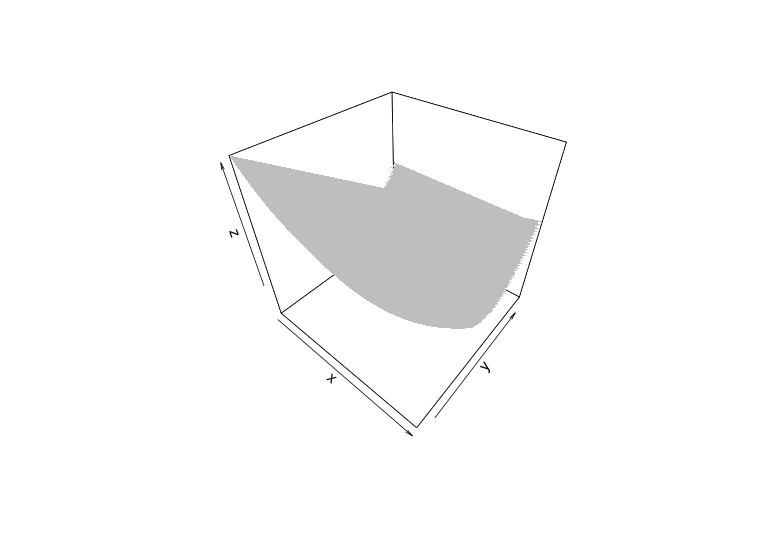
\includegraphics[scale=0.4]{plot3d.png}
\end{center}
\caption{\(x=b0,y=b1,z=mse(b0,b1)\)}
\end{figure}
Hopefully the plot will be more clear on R

{\centering \section*{Second Question}}
{\centering\subsection*{A}}
To be able to decide how the size confidence intervals depend on number of observation and confidence level, am going to change confidence level for 2 sets , after that change number of observation.That's to get better thought about what's happening.\\
\begin{tabular}{|c|c|c|c|}
	\hline
	Set&\(y_0\)&\(n\)&confidence.level\\
	\hline
	1&0&100&0.3\\
	\hline
	2&0&100&0.8\\
	\hline
	3&0&200&0.5\\
	\hline
	4&0&50&0.5\\
	\hline
\end{tabular}\\
\textbf{Note:}I didn't change \(y_0\) because It will change only the center the rest will stay the same.
\begin{flushleft}
The plots where as following :
\begin{figure}[H]
\begin{center}
	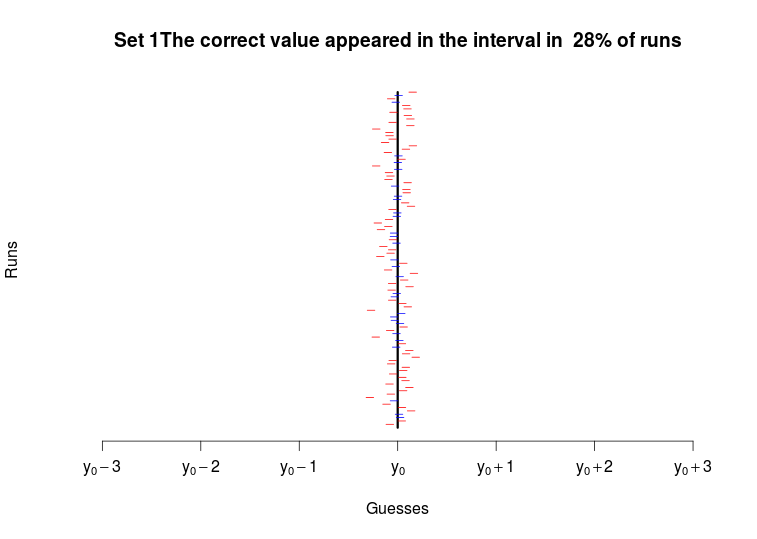
\includegraphics[scale=0.3]{plotset1.png}
\end{center}
\caption{Set 1 }
\end{figure}
Between figure 3 \& figure 4 (Set 1 \& Set 2)the only thing that change is confidence level and we can notice that it really affected the result.
\begin{figure}[H]
	\begin{center}
		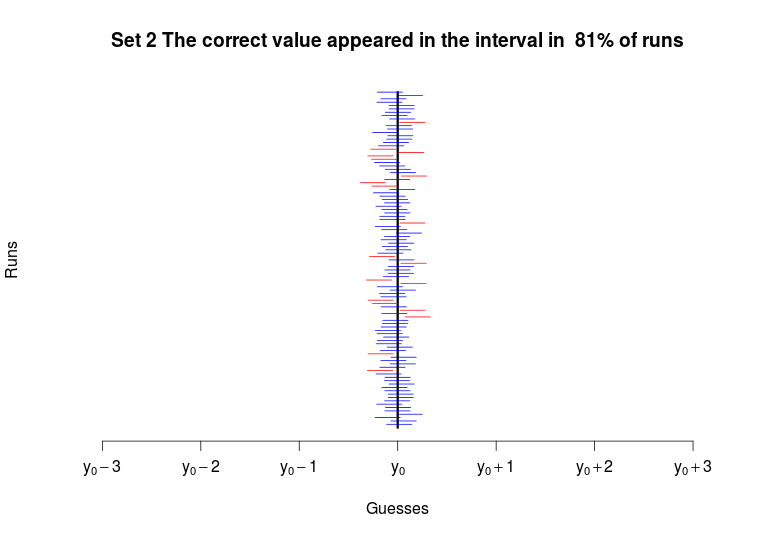
\includegraphics[scale=0.3]{plotset2.png}
	\end{center}
	\caption{Set 2 }
\end{figure}
\begin{figure}[H]
	\begin{center}
		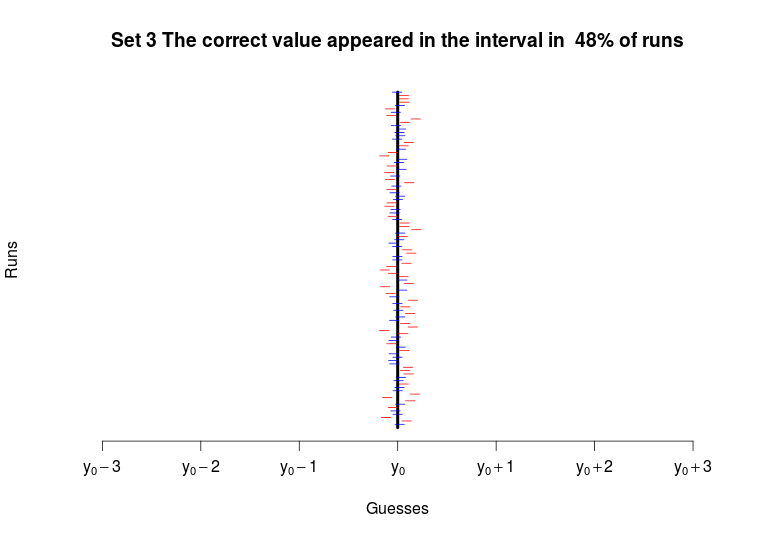
\includegraphics[scale=0.3]{plotset3.png}
	\end{center}
	\caption{Set 3 }
\end{figure}
I don't know if I am lucky to get figure 5 \& figure 6 (set 3 \& set 4) the same percentage on both of them.Anyway this show that the size of data doesn't have an effect or less effect.
\begin{figure}[H]
	\begin{center}
		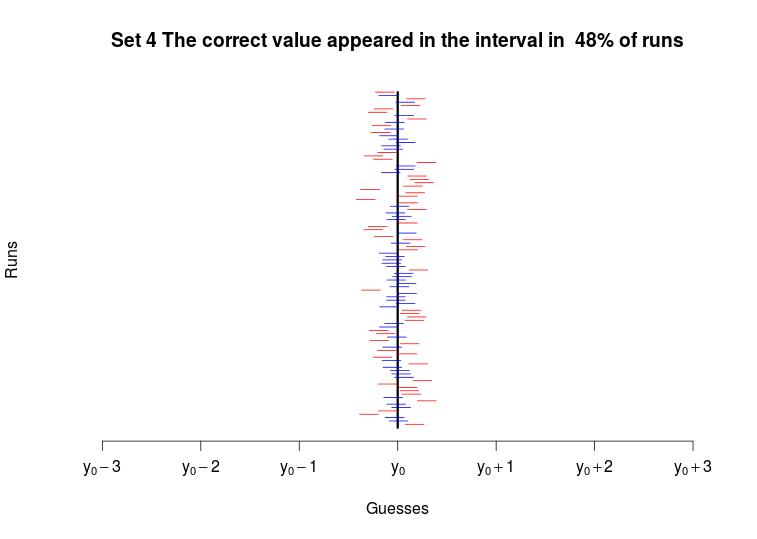
\includegraphics[scale=0.3]{plotset4.png}
	\end{center}
	\caption{Set 4 }
\end{figure}
\textbf{Note:}I tried to used larger \(n\) or observations but the plot got very small and crowded.
In first plot in the first algorithm the probability that \(y_0\) in the interval is 0.28 since it appeared in 28\% of the intervals.

{\centering\subsection*{B}}
The first way of measurement it's already implemented in the file, were we consider each data generated cost 0.05 cents and 1 Euro for each measurement in the interval, here is the code :
\begin{lstlisting}[language=R]
n <- c()
cost <- c()
success <- c()
for(k in c(1:20)){
y0 <- runif(1, min = -100, max = 100)

# We use a measurements strategy where we make randomly 2, ..., 100 low precision measurements 
n[k] <- sample(c(2:100), 1)
y <- GenerateData(y0, n[k])
cost[k] <- 0.05 * n[k]

# Lets estimate the interval for confidence level 50%
interval <- GetConfidenceInterval(y, 0.50)
cost[k] <- cost[k] + 1 * (interval[2] - interval[1])

# Lets see whether the high precision scan was successful or not
success[k] <- (interval[1] <= y0) && (y0 <= interval[2]) 
}
par(mfrow = c(2, 2))
barplot(n, space = 0.1, col = c("red", "blue")[1 + success], ylab = "Number of measurements", ylim=c(0, 100),  xlab = "Run")
barplot(0.05 * n, space = 0.1, col = c("red", "blue")[1 + success], ylab = "Cost of low-quality measurements", ylim=c(0, 5),  xlab = "Run")
barplot(cost - 0.05 * n, space = 0.1, col = c("red", "blue")[1 + success], ylab = "Cost of high-quality scan", xlab = "Run")
barplot(cost, space = 0.1, col = c("red", "blue")[1 + success], ylab = "Overall cost", ylim = c(0,10), xlab = "Run")

par(mfrow = c(1, 2))
barplot(n, space = 0.1, col = c("red", "blue")[1 + success], ylab = "Number of measurements", ylim=c(0, 100),  xlab = "Run")
plot(cumsum(cost)/cumsum(success), type = "s", xlab = "Run", ylab = "Average cost")
\end{lstlisting}
From the previous code we get two plots (figure 7 \& figure 8)
\begin{figure}[H]
\begin{center}
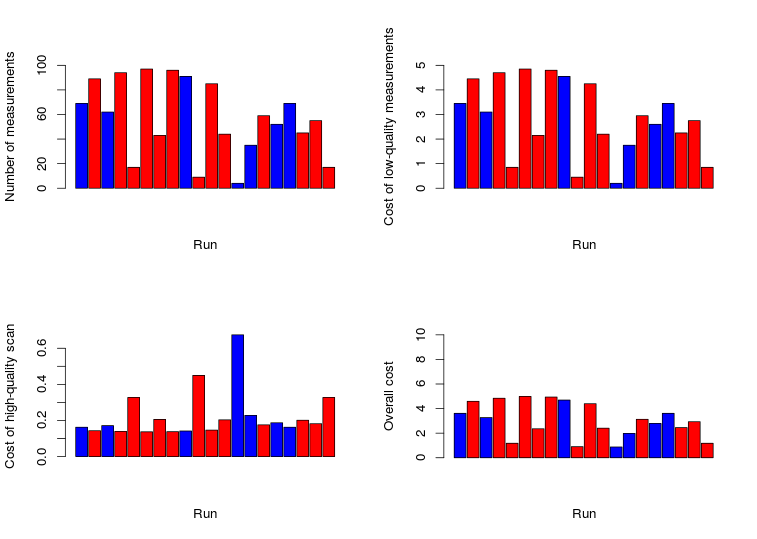
\includegraphics[scale=0.3]{plotm1p1.png}
\end{center}
\caption{Plots show variables in each run}
\end{figure}
What I noticed from figure 7 is:
\begin{enumerate}
	\item The more measurements we have, the more low-quality cost.
	\item More measurements mean less high-quality cost.
	\item The overall estimation is the more measurements the more cost.
\end{enumerate}
\begin{figure}[H]
	\begin{center}
		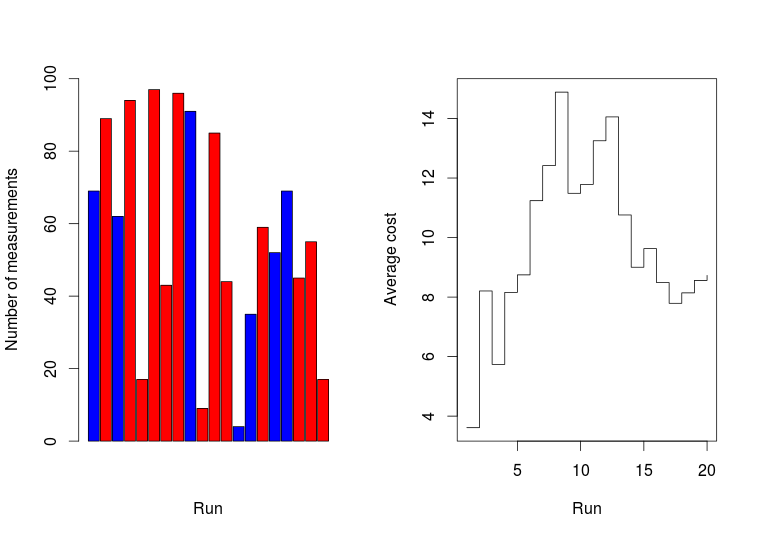
\includegraphics[scale=0.3]{plotm1p2.png}
	\end{center}
	\caption{Plots show variables in each run}
\end{figure}
Figure 8 also assure the results we got from figure 7.
Actually my head went blank for another strategy and there was non-answered question on the forum about this question as well.Anyway  I thought about playing with the confidence level to make it random as well between 0.1,0.9 and check how that is going to affect.
The code become like this :
\begin{lstlisting}[language=R]
n <- c()
cost <- c()
success <- c()
precision<-c()
for(k in c(1:20)){
y0 <- runif(1, min = -100, max = 100)

# We use a measurements strategy where we make randomly 2, ..., 100 low precision measurements 
n[k] <- sample(c(2:100), 1)
y <- GenerateData(y0, n[k])
cost[k] <- 0.05 * n[k]

# Lets estimate the interval for confidence level 50%
?sample
precision[k]<-sample(seq(0.1,0.9,0.1),1)
interval <- GetConfidenceInterval(y, precision[k])
cost[k] <- cost[k] + 1 * (interval[2] - interval[1])

# Lets see whether the high precision scan was successful or not
success[k] <- (interval[1] <= y0) && (y0 <= interval[2]) 

}
barplot(precision, space = 0.1, col = c("red", "blue")[1 + success], ylab = "Confidience Level", ylim=c(0, 1),  xlab = "Run")
par(mfrow = c(2, 2))
barplot(n, space = 0.1, col = c("red", "blue")[1 + success], ylab = "Number of measurements", ylim=c(0, 100),  xlab = "Run")
barplot(0.05 * n, space = 0.1, col = c("red", "blue")[1 + success], ylab = "Cost of low-quality measurements", ylim=c(0, 5),  xlab = "Run")
barplot(cost - 0.05 * n, space = 0.1, col = c("red", "blue")[1 + success], ylab = "Cost of high-quality scan", xlab = "Run")
barplot(cost, space = 0.1, col = c("red", "blue")[1 + success], ylab = "Overall cost", ylim = c(0,10), xlab = "Run")

par(mfrow = c(1, 2))
barplot(n, space = 0.1, col = c("red", "blue")[1 + success], ylab = "Number of measurements", ylim=c(0, 100),  xlab = "Run")
plot(cumsum(cost)/cumsum(success), type = "s", xlab = "Run", ylab = "Average cost")
\end{lstlisting}
And the figures are : 
\begin{figure}[H]
\begin{center}
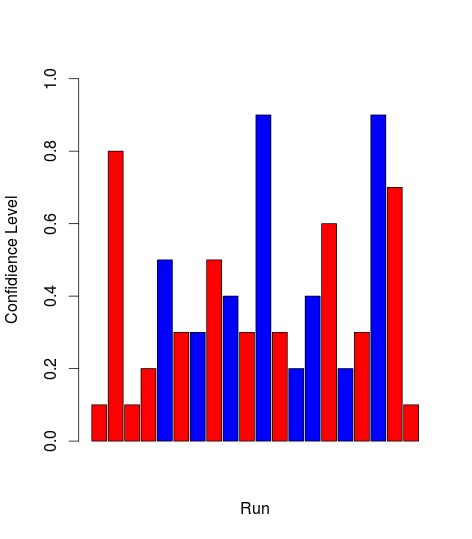
\includegraphics[scale=0.4]{plotm2confidence.png}
\end{center}
\caption{Shows the confidence level over the runs}
\end{figure}

\begin{figure}[H]
	\begin{center}
		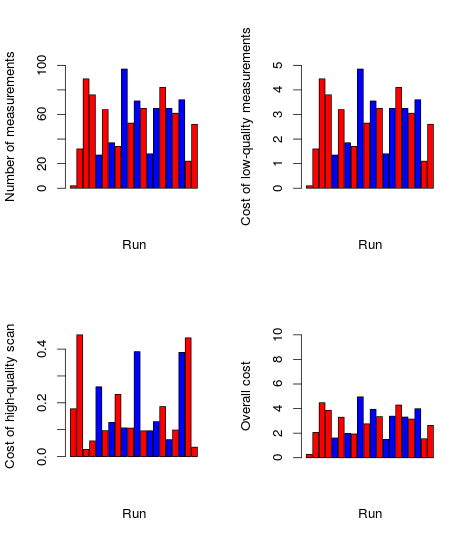
\includegraphics[scale=0.5]{plotm2p1.png}
	\end{center}
	\caption{Shows the variables over the runs}
\end{figure}

\begin{figure}[H]
	\begin{center}
		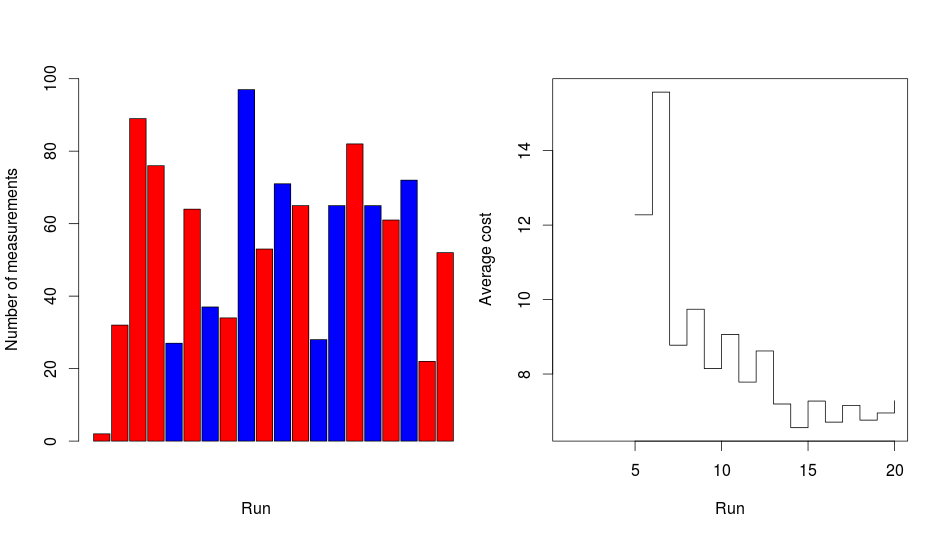
\includegraphics[scale=0.2]{plotm2p2.png}
	\end{center}
	\caption{Shows the variables over the runs}
\end{figure}
\textbf{Conclusion:} I conclude that the number of measurements has it's effect on the total cost.In the other hand confidence doesn't have any effect on the cost.
\end{flushleft}
{\centering \section*{Third Question}}
{\centering\subsection*{A}}
\begin{flushleft}

For quadratic model \(x_1 = x,x_2 = x^2\) , and for the first task it's already implemented in the file by this code:
\begin{lstlisting}[language=R]

# Let prepare the extended data matrix for fitting quadratic relations y ~ x^2 + x + 1
quadratic.data <- data.frame(x1 = data$x, x2 = data$x^2, y = data$y)

plot(data$x, predict(lm(y~x1+x2+1, quadratic.data), newdata = quadratic.data), type="l", col="red")
points(data, pch=16)
coef(lm(y~x1+x2+1, quadratic.data))
\end{lstlisting}
The output for the previous code is the following figure 12:
\begin{figure}[H]
\begin{center}
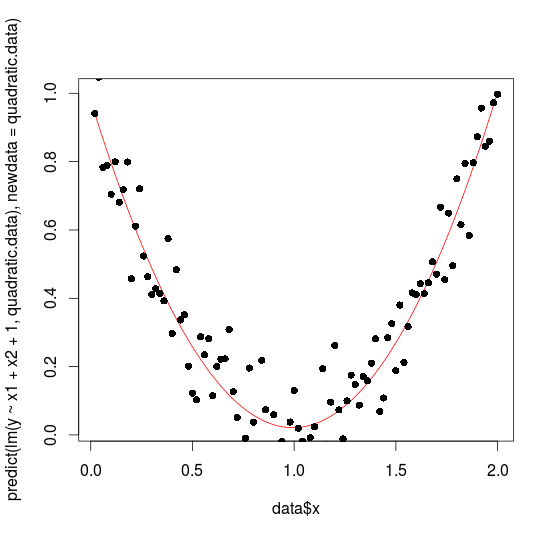
\includegraphics[scale=0.4]{plotquaratic.png}
\end{center}
\caption{Shows the quadratic formula over the points}
\end{figure}
The coefficient was \(intercepter = 0.9792486 ,x1=-1.9281042,x2 =0.9701058\) \\
For degree of 10 I used the following code : 
\begin{lstlisting}[language=R]
# Lets prepare the extended datamatrix for fitting polynomials with degree 10
deg10.data <- data.frame(x1 = data$x, x2 = data$x^2,x3=data$x^3,x4=data$x^4,x5=data$x^5,
x6=data$x^6,x7=data$x^7,x8=data$x^8,x9=data$x^9,x10=data$x^10, y = data$y)
plot(data$x, predict(lm(y~x1+x2+x3+x4+x5+x6+x7+x8+x9+x10+1, deg10.data ), newdata = deg10.data), type="l", col="red")
points(data, pch=16)
\end{lstlisting}
The figure was as following : 
\begin{figure}[H]
\begin{center}
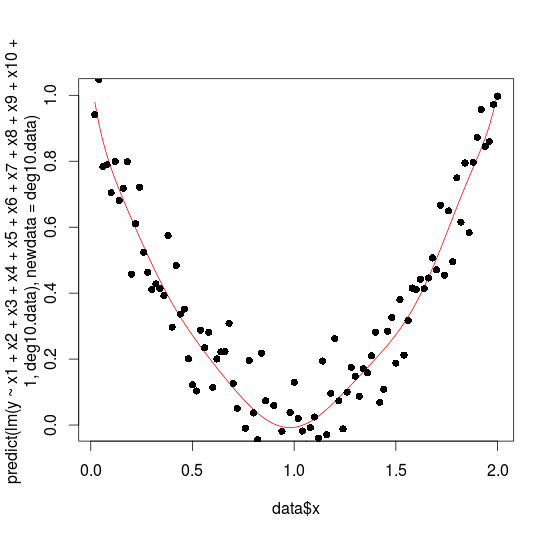
\includegraphics[scale=0.3]{plotdeg10.png}
\end{center}
\caption{Show the degree 10 polynomial with points}
\end{figure}
Comparing deg10 to quadratic actually they looked the same at first but after magnifying looks like deg10 has more has curves.\\
Also I compared the result of all the ways to calculate the coefficients and I got the same result ( just to make sure that am on the right track).Here is the code:
\begin{lstlisting}[language=R]
coef(lm(y~x1+x2+x3+x4+x5+x6+x7+x8+x9+x10+1, deg10.data))
coef(lm(y~.,data = deg10.data))
coef(lm(y~poly(x,10,raw=TRUE),data = data))
\end{lstlisting}
\end{flushleft}
{\centering\subsection*{B}}
{\centering \section*{Fourth Question}}
{\centering\subsection*{A}}
{\centering\subsection*{B}}
{\centering \section*{Fifth Question}}
{\centering\subsection*{A}}
{\centering\subsection*{B}}
{\centering\subsection*{C}}
{\centering\subsection*{D}}
{\centering \section*{Sixth Question}}

\end{flushleft}
		\end{multicols*}
\end{document}